\documentclass[tikz,border=0mm]{standalone}
\usepackage[utf8]{inputenc}
\usepackage{unicode-math} % for unicode support in math environments
\usepackage{amsmath}
\usepackage{siunitx}
\usepackage{booktabs}
\sisetup{mode=text,range-phrase = {\text{~to~}}, range-units=single, print-unity-mantissa=false}
\usepackage{mhchem}
\usepackage{tikz}



\usepackage{fontspec}

\directlua{
  luaotfload.add_fallback(
  "FallbackFonts",
  {
        "DejaVu Serif:mode=harf;",
        "DejaVu Sans Mono:mode=harf;",
        % we could add many more fonts here optionally!
    }
  )
}

\setmainfont{CMU Serif}[RawFeature={fallback=FallbackFonts}]
\setmonofont{Inconsolata}[RawFeature={fallback=FallbackFonts}]

\begin{document}
\definecolor{backgroundColor}{rgb}{1.0, 1.0, 1.0}

\pagecolor{backgroundColor}


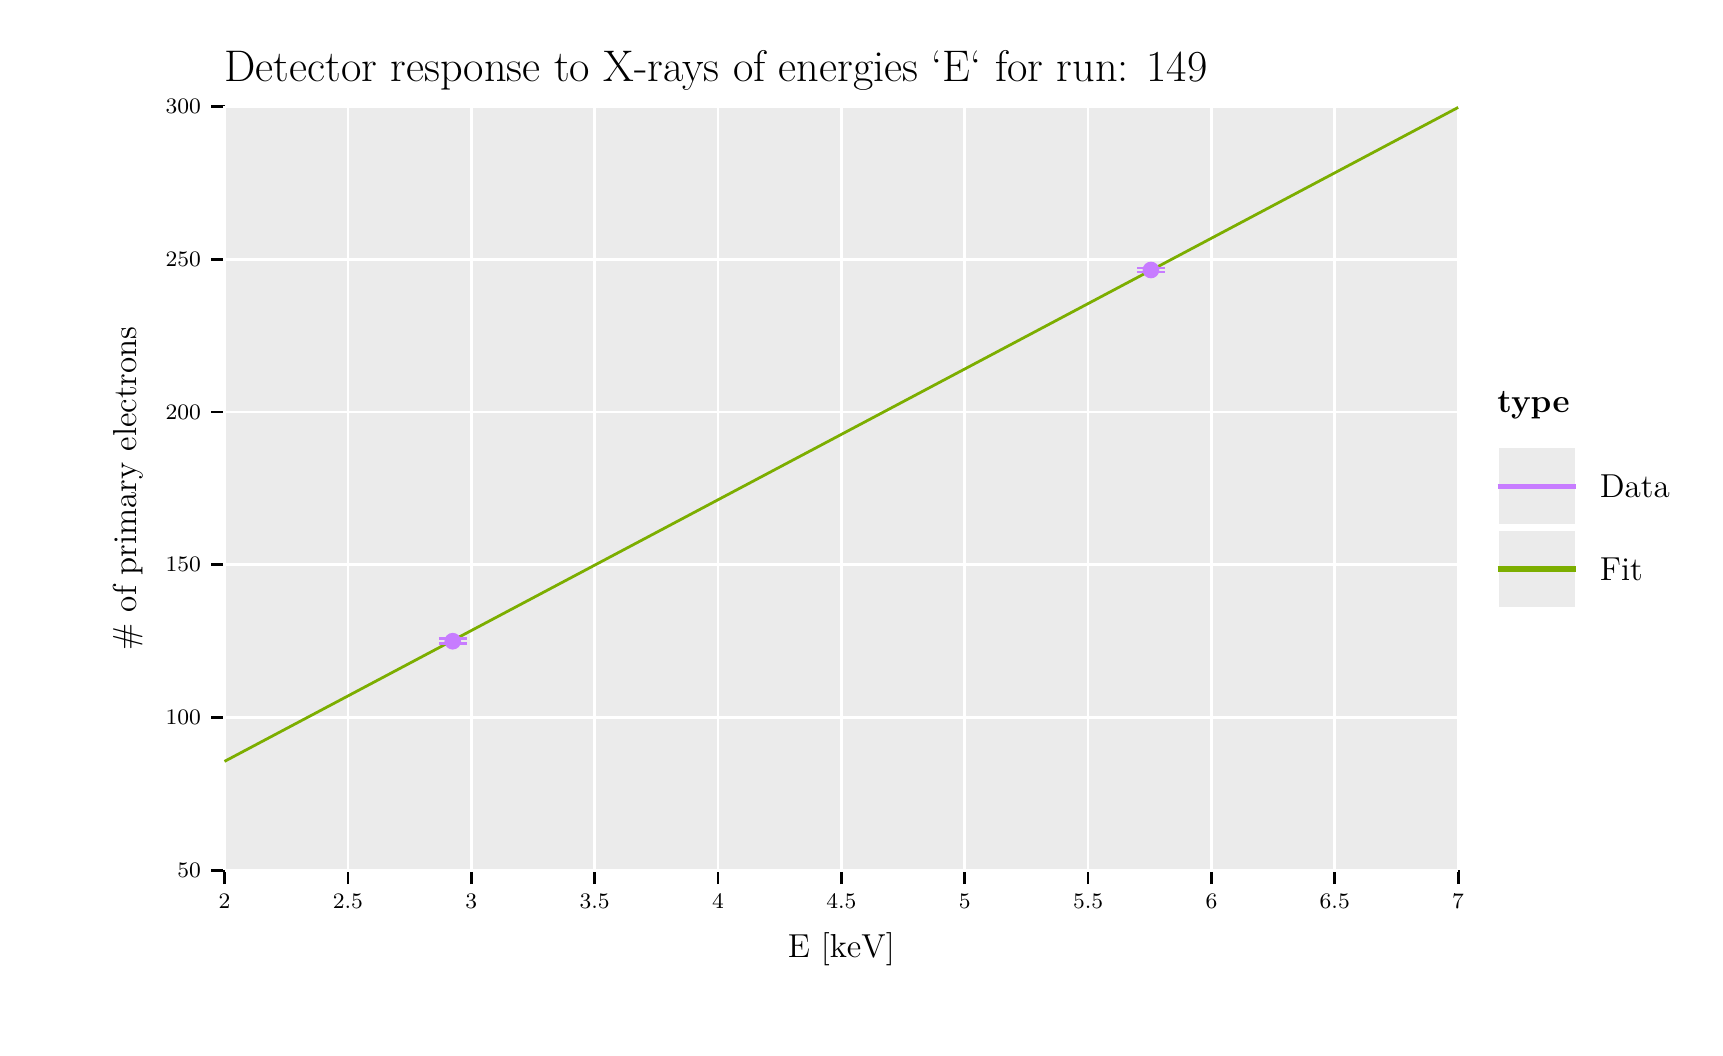
\begin{tikzpicture}[every node/.style={outer sep=0pt, inner sep=0pt}]
\path[use as bounding box] (0, 0) rectangle (600.0bp, 360.0bp) ;
\definecolor{drawColor}{rgb}{0.0, 0.0, 0.0}
\definecolor{fillColor}{rgb}{1.0, 1.0, 1.0}

\draw [color = drawColor, fill = fillColor, draw opacity = 0.0, fill opacity = 1.0, line width = 0.0bp] (0.0000bp, 360.0000bp) rectangle (600.0000bp, 0.0000bp) ;
\node [right, font=\fontsize{16.0}{19.2}\selectfont
, anchor=west] at (70.8661bp, 344.4711bp){Detector response to X-rays of energies `E` for run: 149} ;
\definecolor{drawColor}{rgb}{0.0, 0.0, 0.0}
\definecolor{fillColor}{rgb}{0.9200000166893005, 0.9200000166893005, 0.9200000166893005}

\draw [color = drawColor, fill = fillColor, draw opacity = 0.0, fill opacity = 1.0, line width = 0.0bp] (70.8661bp, 331.6535bp) rectangle (514.9606bp, 56.6929bp) ;
\definecolor{drawColor}{rgb}{0.0, 0.0, 0.0}
\definecolor{fillColor}{rgb}{0.0, 0.0, 0.0}

\draw [color = drawColor, fill = fillColor, draw opacity = 1.0, fill opacity = 0.0, line width = 1.0bp] (70.8661bp, 51.6929bp)--(70.8661bp, 56.6929bp) ;
\draw [color = drawColor, fill = fillColor, draw opacity = 1.0, fill opacity = 0.0, line width = 1.0bp] (115.2756bp, 51.6929bp)--(115.2756bp, 56.6929bp) ;
\draw [color = drawColor, fill = fillColor, draw opacity = 1.0, fill opacity = 0.0, line width = 1.0bp] (159.6850bp, 51.6929bp)--(159.6850bp, 56.6929bp) ;
\draw [color = drawColor, fill = fillColor, draw opacity = 1.0, fill opacity = 0.0, line width = 1.0bp] (204.0945bp, 51.6929bp)--(204.0945bp, 56.6929bp) ;
\draw [color = drawColor, fill = fillColor, draw opacity = 1.0, fill opacity = 0.0, line width = 1.0bp] (248.5039bp, 51.6929bp)--(248.5039bp, 56.6929bp) ;
\draw [color = drawColor, fill = fillColor, draw opacity = 1.0, fill opacity = 0.0, line width = 1.0bp] (292.9134bp, 51.6929bp)--(292.9134bp, 56.6929bp) ;
\draw [color = drawColor, fill = fillColor, draw opacity = 1.0, fill opacity = 0.0, line width = 1.0bp] (337.3228bp, 51.6929bp)--(337.3228bp, 56.6929bp) ;
\draw [color = drawColor, fill = fillColor, draw opacity = 1.0, fill opacity = 0.0, line width = 1.0bp] (381.7323bp, 51.6929bp)--(381.7323bp, 56.6929bp) ;
\draw [color = drawColor, fill = fillColor, draw opacity = 1.0, fill opacity = 0.0, line width = 1.0bp] (426.1417bp, 51.6929bp)--(426.1417bp, 56.6929bp) ;
\draw [color = drawColor, fill = fillColor, draw opacity = 1.0, fill opacity = 0.0, line width = 1.0bp] (470.5512bp, 51.6929bp)--(470.5512bp, 56.6929bp) ;
\draw [color = drawColor, fill = fillColor, draw opacity = 1.0, fill opacity = 0.0, line width = 1.0bp] (514.9606bp, 51.6929bp)--(514.9606bp, 56.6929bp) ;
\node [font=\fontsize{8.0}{9.6}\selectfont
] at (70.8661bp, 45.5272bp){2} ;
\node [font=\fontsize{8.0}{9.6}\selectfont
] at (115.2756bp, 45.4389bp){2.5} ;
\node [font=\fontsize{8.0}{9.6}\selectfont
] at (159.6850bp, 45.4389bp){3} ;
\node [font=\fontsize{8.0}{9.6}\selectfont
] at (204.0945bp, 45.4389bp){3.5} ;
\node [font=\fontsize{8.0}{9.6}\selectfont
] at (248.5039bp, 45.4830bp){4} ;
\node [font=\fontsize{8.0}{9.6}\selectfont
] at (292.9134bp, 45.3947bp){4.5} ;
\node [font=\fontsize{8.0}{9.6}\selectfont
] at (337.3228bp, 45.4389bp){5} ;
\node [font=\fontsize{8.0}{9.6}\selectfont
] at (381.7323bp, 45.4389bp){5.5} ;
\node [font=\fontsize{8.0}{9.6}\selectfont
] at (426.1417bp, 45.4389bp){6} ;
\node [font=\fontsize{8.0}{9.6}\selectfont
] at (470.5512bp, 45.4389bp){6.5} ;
\node [font=\fontsize{8.0}{9.6}\selectfont
] at (514.9606bp, 45.3987bp){7} ;
\draw [color = drawColor, fill = fillColor, draw opacity = 1.0, fill opacity = 0.0, line width = 1.0bp] (70.8661bp, 56.6929bp)--(65.8661bp, 56.6929bp) ;
\draw [color = drawColor, fill = fillColor, draw opacity = 1.0, fill opacity = 0.0, line width = 1.0bp] (70.8661bp, 111.6850bp)--(65.8661bp, 111.6850bp) ;
\draw [color = drawColor, fill = fillColor, draw opacity = 1.0, fill opacity = 0.0, line width = 1.0bp] (70.8661bp, 166.6772bp)--(65.8661bp, 166.6772bp) ;
\draw [color = drawColor, fill = fillColor, draw opacity = 1.0, fill opacity = 0.0, line width = 1.0bp] (70.8661bp, 221.6693bp)--(65.8661bp, 221.6693bp) ;
\draw [color = drawColor, fill = fillColor, draw opacity = 1.0, fill opacity = 0.0, line width = 1.0bp] (70.8661bp, 276.6614bp)--(65.8661bp, 276.6614bp) ;
\draw [color = drawColor, fill = fillColor, draw opacity = 1.0, fill opacity = 0.0, line width = 1.0bp] (70.8661bp, 331.6535bp)--(65.8661bp, 331.6535bp) ;
\node [left, font=\fontsize{8.0}{9.6}\selectfont
, anchor=east] at (62.3744bp, 56.6929bp){50} ;
\node [left, font=\fontsize{8.0}{9.6}\selectfont
, anchor=east] at (62.3744bp, 111.6850bp){100} ;
\node [left, font=\fontsize{8.0}{9.6}\selectfont
, anchor=east] at (62.3744bp, 166.6772bp){150} ;
\node [left, font=\fontsize{8.0}{9.6}\selectfont
, anchor=east] at (62.3744bp, 221.6693bp){200} ;
\node [left, font=\fontsize{8.0}{9.6}\selectfont
, anchor=east] at (62.3744bp, 276.6614bp){250} ;
\node [left, font=\fontsize{8.0}{9.6}\selectfont
, anchor=east] at (62.3744bp, 331.6535bp){300} ;
\node [font=\fontsize{12.0}{14.4}\selectfont
] at (292.9134bp, 28.3465bp){E [$\si{keV}$]} ;
\node [rotate = 90.0, font=\fontsize{12.0}{14.4}\selectfont
] at (36.1440bp, 194.1732bp){\# of primary electrons} ;
\definecolor{drawColor}{rgb}{1.0, 1.0, 1.0}
\definecolor{fillColor}{rgb}{0.0, 0.0, 0.0}

\draw [color = drawColor, fill = fillColor, draw opacity = 1.0, fill opacity = 0.0, line width = 1.0bp] (70.8661bp, 331.6535bp)--(70.8661bp, 56.6929bp) ;
\draw [color = drawColor, fill = fillColor, draw opacity = 1.0, fill opacity = 0.0, line width = 1.0bp] (115.2756bp, 331.6535bp)--(115.2756bp, 56.6929bp) ;
\draw [color = drawColor, fill = fillColor, draw opacity = 1.0, fill opacity = 0.0, line width = 1.0bp] (159.6850bp, 331.6535bp)--(159.6850bp, 56.6929bp) ;
\draw [color = drawColor, fill = fillColor, draw opacity = 1.0, fill opacity = 0.0, line width = 1.0bp] (204.0945bp, 331.6535bp)--(204.0945bp, 56.6929bp) ;
\draw [color = drawColor, fill = fillColor, draw opacity = 1.0, fill opacity = 0.0, line width = 1.0bp] (248.5039bp, 331.6535bp)--(248.5039bp, 56.6929bp) ;
\draw [color = drawColor, fill = fillColor, draw opacity = 1.0, fill opacity = 0.0, line width = 1.0bp] (292.9134bp, 331.6535bp)--(292.9134bp, 56.6929bp) ;
\draw [color = drawColor, fill = fillColor, draw opacity = 1.0, fill opacity = 0.0, line width = 1.0bp] (337.3228bp, 331.6535bp)--(337.3228bp, 56.6929bp) ;
\draw [color = drawColor, fill = fillColor, draw opacity = 1.0, fill opacity = 0.0, line width = 1.0bp] (381.7323bp, 331.6535bp)--(381.7323bp, 56.6929bp) ;
\draw [color = drawColor, fill = fillColor, draw opacity = 1.0, fill opacity = 0.0, line width = 1.0bp] (426.1417bp, 331.6535bp)--(426.1417bp, 56.6929bp) ;
\draw [color = drawColor, fill = fillColor, draw opacity = 1.0, fill opacity = 0.0, line width = 1.0bp] (470.5512bp, 331.6535bp)--(470.5512bp, 56.6929bp) ;
\draw [color = drawColor, fill = fillColor, draw opacity = 1.0, fill opacity = 0.0, line width = 1.0bp] (514.9606bp, 331.6535bp)--(514.9606bp, 56.6929bp) ;
\draw [color = drawColor, fill = fillColor, draw opacity = 1.0, fill opacity = 0.0, line width = 1.0bp] (70.8661bp, 56.6929bp)--(514.9606bp, 56.6929bp) ;
\draw [color = drawColor, fill = fillColor, draw opacity = 1.0, fill opacity = 0.0, line width = 1.0bp] (70.8661bp, 111.6850bp)--(514.9606bp, 111.6850bp) ;
\draw [color = drawColor, fill = fillColor, draw opacity = 1.0, fill opacity = 0.0, line width = 1.0bp] (70.8661bp, 166.6772bp)--(514.9606bp, 166.6772bp) ;
\draw [color = drawColor, fill = fillColor, draw opacity = 1.0, fill opacity = 0.0, line width = 1.0bp] (70.8661bp, 221.6693bp)--(514.9606bp, 221.6693bp) ;
\draw [color = drawColor, fill = fillColor, draw opacity = 1.0, fill opacity = 0.0, line width = 1.0bp] (70.8661bp, 276.6614bp)--(514.9606bp, 276.6614bp) ;
\draw [color = drawColor, fill = fillColor, draw opacity = 1.0, fill opacity = 0.0, line width = 1.0bp] (70.8661bp, 331.6535bp)--(514.9606bp, 331.6535bp) ;
\definecolor{drawColor}{rgb}{0.4848798215389252, 0.683388352394104, 0.0}
\definecolor{fillColor}{rgb}{0.0, 0.0, 0.0}

\draw [color = drawColor, fill = fillColor, draw opacity = 1.0, fill opacity = 0.0, line width = 1.0bp]
(70.8661bp, 95.8653bp)  -- 
(75.3519bp, 98.2432bp)  -- 
(79.8377bp, 100.6211bp)  -- 
(84.3236bp, 102.9990bp)  -- 
(88.8094bp, 105.3769bp)  -- 
(93.2952bp, 107.7548bp)  -- 
(97.7810bp, 110.1327bp)  -- 
(102.2668bp, 112.5106bp)  -- 
(106.7526bp, 114.8885bp)  -- 
(111.2384bp, 117.2664bp)  -- 
(115.7242bp, 119.6443bp)  -- 
(120.2100bp, 122.0222bp)  -- 
(124.6958bp, 124.4001bp)  -- 
(129.1816bp, 126.7780bp)  -- 
(133.6674bp, 129.1558bp)  -- 
(138.1532bp, 131.5337bp)  -- 
(142.6390bp, 133.9116bp)  -- 
(147.1248bp, 136.2895bp)  -- 
(151.6106bp, 138.6674bp)  -- 
(156.0964bp, 141.0453bp)  -- 
(160.5822bp, 143.4232bp)  -- 
(165.0680bp, 145.8011bp)  -- 
(169.5538bp, 148.1790bp)  -- 
(174.0396bp, 150.5569bp)  -- 
(178.5254bp, 152.9348bp)  -- 
(183.0112bp, 155.3127bp)  -- 
(187.4970bp, 157.6906bp)  -- 
(191.9828bp, 160.0685bp)  -- 
(196.4686bp, 162.4463bp)  -- 
(200.9544bp, 164.8242bp)  -- 
(205.4402bp, 167.2021bp)  -- 
(209.9260bp, 169.5800bp)  -- 
(214.4118bp, 171.9579bp)  -- 
(218.8976bp, 174.3358bp)  -- 
(223.3834bp, 176.7137bp)  -- 
(227.8692bp, 179.0916bp)  -- 
(232.3550bp, 181.4695bp)  -- 
(236.8408bp, 183.8474bp)  -- 
(241.3267bp, 186.2253bp)  -- 
(245.8125bp, 188.6032bp)  -- 
(250.2983bp, 190.9811bp)  -- 
(254.7841bp, 193.3590bp)  -- 
(259.2699bp, 195.7368bp)  -- 
(263.7557bp, 198.1147bp)  -- 
(268.2415bp, 200.4926bp)  -- 
(272.7273bp, 202.8705bp)  -- 
(277.2131bp, 205.2484bp)  -- 
(281.6989bp, 207.6263bp)  -- 
(286.1847bp, 210.0042bp)  -- 
(290.6705bp, 212.3821bp)  -- 
(295.1563bp, 214.7600bp)  -- 
(299.6421bp, 217.1379bp)  -- 
(304.1279bp, 219.5158bp)  -- 
(308.6137bp, 221.8937bp)  -- 
(313.0995bp, 224.2716bp)  -- 
(317.5853bp, 226.6495bp)  -- 
(322.0711bp, 229.0273bp)  -- 
(326.5569bp, 231.4052bp)  -- 
(331.0427bp, 233.7831bp)  -- 
(335.5285bp, 236.1610bp)  -- 
(340.0143bp, 238.5389bp)  -- 
(344.5001bp, 240.9168bp)  -- 
(348.9859bp, 243.2947bp)  -- 
(353.4717bp, 245.6726bp)  -- 
(357.9575bp, 248.0505bp)  -- 
(362.4433bp, 250.4284bp)  -- 
(366.9291bp, 252.8063bp)  -- 
(371.4149bp, 255.1842bp)  -- 
(375.9007bp, 257.5621bp)  -- 
(380.3865bp, 259.9400bp)  -- 
(384.8723bp, 262.3178bp)  -- 
(389.3581bp, 264.6957bp)  -- 
(393.8440bp, 267.0736bp)  -- 
(398.3298bp, 269.4515bp)  -- 
(402.8156bp, 271.8294bp)  -- 
(407.3014bp, 274.2073bp)  -- 
(411.7872bp, 276.5852bp)  -- 
(416.2730bp, 278.9631bp)  -- 
(420.7588bp, 281.3410bp)  -- 
(425.2446bp, 283.7189bp)  -- 
(429.7304bp, 286.0968bp)  -- 
(434.2162bp, 288.4747bp)  -- 
(438.7020bp, 290.8526bp)  -- 
(443.1878bp, 293.2305bp)  -- 
(447.6736bp, 295.6083bp)  -- 
(452.1594bp, 297.9862bp)  -- 
(456.6452bp, 300.3641bp)  -- 
(461.1310bp, 302.7420bp)  -- 
(465.6168bp, 305.1199bp)  -- 
(470.1026bp, 307.4978bp)  -- 
(474.5884bp, 309.8757bp)  -- 
(479.0742bp, 312.2536bp)  -- 
(483.5600bp, 314.6315bp)  -- 
(488.0458bp, 317.0094bp)  -- 
(492.5316bp, 319.3873bp)  -- 
(497.0174bp, 321.7652bp)  -- 
(501.5032bp, 324.1431bp)  -- 
(505.9890bp, 326.5210bp)  -- 
(510.4748bp, 328.8988bp)  -- 
(514.9606bp, 331.2767bp)
;\definecolor{drawColor}{rgb}{0.7804079055786133, 0.4866028726100922, 1.0}
\definecolor{fillColor}{rgb}{0.0, 0.0, 0.0}

\draw [color = drawColor, fill = fillColor, draw opacity = 1.0, fill opacity = 0.0, line width = 1.0bp] (153.0236bp, 139.9611bp)--(153.0236bp, 138.2811bp) ;
\draw [color = drawColor, fill = fillColor, draw opacity = 1.0, fill opacity = 0.0, line width = 1.0bp] (148.0236bp, 139.9611bp)--(158.0236bp, 139.9611bp) ;
\draw [color = drawColor, fill = fillColor, draw opacity = 1.0, fill opacity = 0.0, line width = 1.0bp] (148.0236bp, 138.2811bp)--(158.0236bp, 138.2811bp) ;
\draw [color = drawColor, fill = fillColor, draw opacity = 1.0, fill opacity = 0.0, line width = 1.0bp] (404.3811bp, 273.4431bp)--(404.3811bp, 272.0747bp) ;
\draw [color = drawColor, fill = fillColor, draw opacity = 1.0, fill opacity = 0.0, line width = 1.0bp] (399.3811bp, 273.4431bp)--(409.3811bp, 273.4431bp) ;
\draw [color = drawColor, fill = fillColor, draw opacity = 1.0, fill opacity = 0.0, line width = 1.0bp] (399.3811bp, 272.0747bp)--(409.3811bp, 272.0747bp) ;
\definecolor{drawColor}{rgb}{0.0, 0.0, 0.0}
\definecolor{fillColor}{rgb}{0.7804079055786133, 0.4866028726100922, 1.0}

\draw [color = drawColor, fill = fillColor, draw opacity = 0.0, fill opacity = 1.0, line width = 1.0bp] (153.0236bp, 139.1211bp) circle [radius=3.0bp] ;
\draw [color = drawColor, fill = fillColor, draw opacity = 0.0, fill opacity = 1.0, line width = 1.0bp] (404.3811bp, 272.7589bp) circle [radius=3.0bp] ;
\node [right, font=\fontsize{12.0}{14.4}\selectfont
, anchor=west] at (529.1339bp, 223.9370bp){\textbf{type}
} ;
\definecolor{drawColor}{rgb}{1.0, 1.0, 1.0}
\definecolor{fillColor}{rgb}{0.9200000166893005, 0.9200000166893005, 0.9200000166893005}

\draw [color = drawColor, fill = fillColor, draw opacity = 1.0, fill opacity = 1.0, line width = 1.0bp] (529.1339bp, 209.0551bp) rectangle (557.4803bp, 180.7087bp) ;
\definecolor{drawColor}{rgb}{0.7804079055786133, 0.4866028726100922, 1.0}
\definecolor{fillColor}{rgb}{0.0, 0.0, 0.0}

\draw [color = drawColor, fill = fillColor, draw opacity = 1.0, fill opacity = 0.0, line width = 2.0bp] (529.1339bp, 194.8819bp)--(557.4803bp, 194.8819bp) ;
\node [right, font=\fontsize{12.0}{14.4}\selectfont
, anchor=west] at (565.9843bp, 194.8819bp){Data} ;
\definecolor{drawColor}{rgb}{1.0, 1.0, 1.0}
\definecolor{fillColor}{rgb}{0.9200000166893005, 0.9200000166893005, 0.9200000166893005}

\draw [color = drawColor, fill = fillColor, draw opacity = 1.0, fill opacity = 1.0, line width = 1.0bp] (529.1339bp, 179.2913bp) rectangle (557.4803bp, 150.9449bp) ;
\definecolor{drawColor}{rgb}{0.4848798215389252, 0.683388352394104, 0.0}
\definecolor{fillColor}{rgb}{0.0, 0.0, 0.0}

\draw [color = drawColor, fill = fillColor, draw opacity = 1.0, fill opacity = 0.0, line width = 2.0bp] (529.1339bp, 165.1181bp)--(557.4803bp, 165.1181bp) ;
\node [right, font=\fontsize{12.0}{14.4}\selectfont
, anchor=west] at (565.9843bp, 165.1181bp){Fit} ;

\end{tikzpicture}

\end{document}

